% -----------------
% abnTeX2: Modelo de Trabalho Academico (tese de doutorado, dissertacao de
% mestrado e trabalhos monograficos em geral) em conformidade com 
% ABNT NBR 14724:2011: Informacao e documentacao - Trabalhos academicos -
% Apresentacao
% -----------------

\documentclass[
	% -- opções da classe memoir --
	12pt,                     % tamanho da fonte
	openright,                % capítulos começam em pág ímpar (insere página vazia caso preciso)
	oneside,                  % twoside para impressão em verso e anverso. Oposto a oneside
	a4paper,                  % tamanho do papel. 
  % -- opções da classe abntex2 --
	% chapter=TITLE,          % títulos de capítulos convertidos em letras maiúsculas
	% section=TITLE,          % títulos de seções convertidos em letras maiúsculas
	% subsection=TITLE,       % títulos de subseções convertidos em letras maiúsculas
	% subsubsection=TITLE,    % títulos de subsubseções convertidos em letras maiúsculas
  % -- opções do pacote babel --
	english,                  % idioma adicional para hifenização
	brazil                    % o último idioma é o principal do documento
]{abntex2}

% --- 
% Pacotes básicos 
\usepackage{lmodern}          % Usa a fonte Latin Modern		>
\usepackage[T1]{fontenc}      % Selecao de codigos de fonte.
\usepackage[utf8]{inputenc}   % Codificacao do documento (conversão automática dos acentos)
\usepackage{lastpage}         % Usado pela Ficha catalográfica
\usepackage{indentfirst}      % Indenta o primeiro parágrafo de cada seção.
\usepackage{color}            % Controle das cores
\usepackage{graphicx}         % Inclusão de gráficos
\usepackage{microtype}        % para melhorias de justificação
\usepackage{colortbl}         % Colorir linhas de tabelas
\usepackage[portuges]{datetime2}
% \DTMlangsetup[portuges]{showdayofmonth=false}
		
% ---
% Pacotes adicionais, usados apenas no âmbito do Modelo Canônico do abnteX2
\usepackage{lipsum}                           % para geração de dummy text

% ---
% Pacotes de citações
\usepackage[brazilian,hyperpageref]{backref}  % Paginas com as citações na bibl
\usepackage[num]{abntex2cite}                 % Citações padrão ABNT

% --- 
% CONFIGURAÇÕES DE PACOTES

% Configurações do pacote backref
% Usado sem a opção hyperpageref de backref
\renewcommand{\backrefpagesname}{Citado na(s) página(s):~}

% Texto padrão antes do número das páginas
\renewcommand{\backref}{}

% Define os textos da citação
\renewcommand*{\backrefalt}[4]{
	\ifcase #1
		Nenhuma citação no texto.
	\or
		Citado na página #2.
	\else
		Citado #1 vezes nas páginas #2.
	\fi}

% Novos comando
\newcommand{\cp}[1]{{\color{orange} [CopyAndPaste] #1}}
\newcommand{\pr}[1]{{\color{blue}[PR] #1}}
\newcommand{\hm}[1]{{\color{red}[HM] #1}}
\newcommand{\todo}[1]{{\color{red}[TO-DO] #1}}

% ---
% Informações de dados para CAPA e FOLHA DE ROSTO

\titulo{Sistema de Monitoramento de Qualidade de Imunobiológicos na Cadeia de Distribuição e Armazenamento}
\autor{Henrique Martins Miranda}
\local{Campina Grande}
\data{\the\year{}}
\orientador{Paulo Ribeiro Lins Junior}
\newcommand{\instituto}{
  Instituto Federal de Educação, Ciência e Tecnologia\\
  da Paraíba - Campus Campina Grande\\
  Curso Superior de Tecnologia em Telemática
}
\tipotrabalho{Trabalho de conclusão de curso}
% O preambulo deve conter o tipo do trabalho, o objetivo, 
% o nome da instituição e a área de concentração 
\preambulo{Monografia apresentada à Coordenação do Curso de Telemática do IFPB - Campus Campina Grande, como requisito parcial para conclusão do curso de Tecnologia em Telemática.}

\renewcommand{\imprimircapa}{
  \begin{capa}
    \center
    
    \begin{figure}
      \begin{center}
        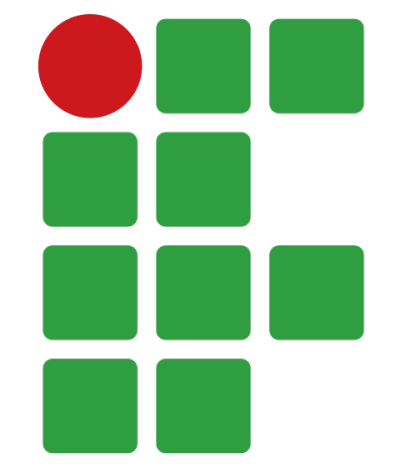
\includegraphics[width=1.8cm]{./assets/logo-ifpb.png}
      \end{center}
    \end{figure}
    
    \ABNTEXchapterfont \large \MakeUppercase{\instituto}
    
    \vspace*{2.5cm}
    
    \ABNTEXchapterfont \large \MakeUppercase{\imprimirautor}
    
    \vfill
    \begin{center}
      \ABNTEXchapterfont \bfseries \large \MakeUppercase{\imprimirtitulo}
    \end{center}
    \vfill
    % \vspace*{6.25cm}

    \large \imprimirlocal
    \par
    \large \imprimirdata
    \vspace*{1cm}
  \end{capa}
}

	
% ---
% Configurações de aparência do PDF final

\definecolor{blue}{RGB}{41,5,195}  % alterando o aspecto da cor azul
\definecolor{orange}{RGB}{255,127,80}

% informações do PDF
\makeatletter
\hypersetup{
  % pagebackref=true,
  pdftitle={\@title}, 
  pdfauthor={\@author},
  pdfsubject={\imprimirpreambulo},
  pdfcreator={LaTeX with abnTeX2},
  pdfkeywords={abnt}{latex}{abntex}{abntex2}{trabalho acadêmico}, 
  colorlinks=true,          % false: boxed links; true: colored links
  linkcolor=black,           % color of internal links
  citecolor=blue,           % color of links to bibliography
  filecolor=magenta,        % color of file links
  urlcolor=black,
  bookmarksdepth=4
}
\makeatother

% --- 
% Espaçamentos entre linhas e parágrafos 

\setlength{\parindent}{1.3cm} % O tamanho do parágrafo

% Controle do espaçamento entre um parágrafo e outro:
\setlength{\parskip}{0.2cm} % Tente também \onelineskip

\makeindex  % Compila o indice

\citebrackets[] % fazer com que as citações dentro do texto virem colchetes

% ---
% Início do documento
\begin{document}
\frenchspacing  % Retira espaço extra obsoleto entre as frases.

% ---
% ELEMENTOS PRÉ-TEXTUAIS
% ---
\pretextual
% \imprimircapa
% \imprimirfolhaderosto*

% % Isto é um exemplo de Ficha Catalográfica, ou ``Dados internacionais de
% catalogação-na-publicação''. Você pode utilizar este modelo como referência. 
% Porém, provavelmente a biblioteca da sua universidade lhe fornecerá um PDF
% com a ficha catalográfica definitiva após a defesa do trabalho. Quando estiver
% com o documento, salve-o como PDF no diretório do seu projeto e substitua todo
% o conteúdo de implementação deste arquivo pelo comando abaixo:
%
% \begin{fichacatalografica}
%     \includepdf{fig_ficha_catalografica.pdf}
% \end{fichacatalografica}

\begin{fichacatalografica}
  \vspace*{\fill}                 % Posição vertical
  \hrule                          % Linha horizontal
  \begin{center}                  % Minipage Centralizado
    \begin{minipage}[c]{12.5cm}   % Largura

      \imprimirautor

      \hspace{0.5cm} \imprimirtitulo  / \imprimirautor. --
      \imprimirlocal, \imprimirdata-

      \hspace{0.5cm} \pageref{LastPage} p. : il. (algumas color.) ; 30 cm.\\

      \hspace{0.5cm} \imprimirorientadorRotulo~\imprimirorientador\\

      \hspace{0.5cm}
      \parbox[t]{\textwidth}{\imprimirtipotrabalho~--~\imprimirinstituicao,
        \imprimirdata.}\\

      \hspace{0.5cm}
      1. Palavra-chave1.
      2. Palavra-chave2.
      I. Orientador.
      II. Universidade xxx.
      III. Faculdade de xxx.
      IV. Título\\

      \hspace{8.75cm} CDU 02:141:005.7\\

    \end{minipage}
  \end{center}
  \hrule
\end{fichacatalografica}
       % Ficha bibliografica
% \begin{errata}
  Elemento opcional da \citeonline[4.2.1.2]{NBR14724:2011}. Exemplo:

  \vspace{\onelineskip}

  FERRIGNO, C. R. A. \textbf{Tratamento de neoplasias ósseas apendiculares com
  reimplantação de enxerto ósseo autólogo autoclavado associado ao plasma
  rico em plaquetas}: estudo crítico na cirurgia de preservação de membro em
  cães. 2011. 128 f. Tese (Livre-Docência) - Faculdade de Medicina Veterinária e
  Zootecnia, Universidade de São Paulo, São Paulo, 2011.

  \begin{table}[htb]
    \center
    \footnotesize
    \begin{tabular}{|p{1.4cm}|p{1cm}|p{3cm}|p{3cm}|}
      \hline
      \textbf{Folha} & \textbf{Linha} & \textbf{Onde se lê} & \textbf{Leia-se} \\
      \hline
      1              & 10             & auto-conclavo       & autoconclavo     \\
      \hline
    \end{tabular}
  \end{table}

\end{errata}
        % Errata
% \begin{folhadeaprovacao}
  \begin{center}
    {\ABNTEXchapterfont\large\imprimirautor}

    \vspace*{\fill}\vspace*{\fill}
    \begin{center}
      \ABNTEXchapterfont \bfseries \Large \imprimirtitulo
    \end{center}
    \vspace*{\fill}

    \hspace{.45\textwidth}
    \begin{minipage}{.5\textwidth}
      \imprimirpreambulo
    \end{minipage}
    \vspace*{\fill}
    
    % Trabalho aprovado. \imprimirlocal, \today:
  \end{center}

  \assinatura{\textbf{\imprimirorientador} \\ Orientador}
  \assinatura{\textbf{Professor} \\ Membro da Banca}
  \assinatura{\textbf{Professor} \\ Membro da Banca}

  \begin{center}
    \vspace*{0.5cm}
    {\large\imprimirlocal}
    \par
    {\large\imprimirdata}
    \vspace*{1cm}
  \end{center}

\end{folhadeaprovacao}
      % Folha de aprovação
% \begin{dedicatoria}
  \vspace*{\fill}
  \centering
  \noindent
  \textit{Este trabalho é dedicado às crianças adultas que,\\
    quando pequenas, sonharam em se tornar cientistas.} \vspace*{\fill}
\end{dedicatoria}
    % Dedicatória
% \begin{agradecimentos}
Agradeço a minha família, amigos e minha namorada, Jennifer Regina, que me ajudaram e deram apoio na construção deste trabalho. Agradeço também a meu amigo Gledson Santos, que participou ativamente no desenvolvimento dos protótipos citados, aos participantes dos laboratórios de pesquisa Assert e GComPI, que fornecerem local e ferramentas para construção dos protótipos e tiram dúvidas de assuntos que não domino, e por fim, agradeço a todos os professores que tive ao longo do curso.
\end{agradecimentos}
        % Agradecimentos
% \begin{epigrafe}
  \vspace*{\fill}
  \begin{flushright}
    \textit{}
  \end{flushright}
\end{epigrafe}
      % Epígrafe
% resumo em português
\setlength{\absparsep}{18pt} % ajusta o espaçamento dos parágrafos do resumo
\begin{resumo}
  O armazenamento é um dos elementos mais importantes da cadeia de distribuição de vacinas, principalmente pela sensibilidade delas às variações de temperatura, que podem ocasionar diminuição da sua eficácia. Considerando isso, existe uma necessidade de manter constante monitoramento dessa variável, a fim de garantir que o produto final venha a manter suas características originais e a eficiência esperada. Esse trabalho apresenta uma solução baseada em Internet das Coisas, usando comunicação sem fio de baixa potência, para monitorar a qualidade de vacinas, por meio das medidas de temperatura e umidade nos locais de armazenamento. Os dados coletados são organizados em um banco de dados, podendo ser acessados por sistemas decisórios com a finalidade de avaliar a qualidade da vacina antes de sua aplicação, evitando transtornos em decorrência de problemas de armazenamento.

  \textbf{Palavras-chaves}: Monitoramento. Vacinas. IoT. LoRa.
\end{resumo}

% resumo em inglês
\begin{resumo}[Abstract]
  \begin{otherlanguage*}{english}
    Storage is one of the most important components of the vaccine distribution chain, mainly due to its sensitivity to temperature variations, which can cause a decrease in its effectiveness. Considering this, there is a need to keep constant monitoring of this variable, to guarantee that the final product will maintain its original characteristics and the expected efficiency. This work presents a solution based on the Internet of Things, using low power wireless communication, to monitor the quality of vaccines, by measuring temperature and humidity in storage locations. The collected data are organized in a database, which can be accessed by decision systems to assess the quality of the vaccine before its application, avoiding problems due to storage problems.

    \noindent
    \textbf{Key-words}: Monitoring. Vacaciones. IoT. LoRa.
  \end{otherlanguage*}
\end{resumo}
     % Resumos
% % ---
% Lista de ilustrações
\pdfbookmark[0]{\listfigurename}{lof}
\listoffigures*
\cleardoublepage

% ---
% Lista de tabelas
\pdfbookmark[0]{\listtablename}{lot}
\listoftables*
\cleardoublepage

% ---
% Lista de abreviaturas e siglas
% \begin{siglas}
%   \item[ABNT] Associação Brasileira de Normas Técnicas
%   \item[abnTeX] ABsurdas Normas para TeX
% \end{siglas}         % Listas

% ---
% Sumario
\pdfbookmark[0]{\contentsname}{toc}
\tableofcontents*
\cleardoublepage

% ---
% ELEMENTOS TEXTUAIS
% ---
\textual

% ---
% Introdução (exemplo de capítulo sem numeração, mas presente no Sumário)
\chapter[Introdução]{Introdução}
\label{cap:intro}
% ---

A saúde é um fator de suma importância para todos os seres vivos, ele é um problema científico, tecnológico, político, prático e filosófico que refere-se a um estado completo de bem estar físico, emocional, social, intelectual e espiritual \cite{almeida2011saude}. 

Segundo o artigo 196 \cite{de2013direito} da Constituição Federal Brasileira a saúde é um direito de todos e dever do Estado garantir medidas políticas sociais e econômicas que visam à diminuição do risco de doenças e de outros agravamentos e ao acesso universal e imparcial às ações e serviços para a sua promoção, proteção e recuperação.

Para garantirmos nossa saúde, precisamos cuidar do nosso corpo e mente, para isto, uma ferramenta que podemos contar são os imunobiológicos, como as vacinas e os soros, diferente de remédios que ajudam no tratamento de pessoas doentes, as imunobiológicos são uma preparação biológica que fornece imunidade total ou parcial de uma determinada doença autoimune para um indivíduo saudável. As vacinas e os soros se diferem pela sua forma de imunização, as vacinas fornece uma imunização ativa, estimulando o nosso organismo na produção de anticorpos, os soros fornecem uma imunização passiva, provendo os anticorpos para o nosso organismo que foram produzidos  em outros organismo \cite{soma2018tratamento}.

Contudo, os imunobiológicos requerem um cuidado elevado para manter a qualidade e sua eficiência, um dos fatores é que são produtos termolábeis, ou seja, se deterioram após determinado tempo expostos a variações de temperaturas e umidade, portanto, é imprescindível assegurar que seu ambiente de armazenagem mantenha uma temperatura e umidade constante \cite{ministerio2001manual} para garantir uma longevidade maior para o produto. Para este propósito, existem a Rede de Frio, um processo desenvolvido pelo Programa Nacional de Imunizações, PNI, de conversação, armazenamento e transporte dos medicamentos, objetivando as condições adequadas dos mesmos, mantendo suas características iniciais \cite{ministerio2001manual}.

No ano de 2014, foi relatado no estudo \cite{oliveira2014avaliaccao} que a qualidade de conservação das vacinas não eram adequadas em boa parte dos municípios da macrorregião Oeste de Minas Gerais, alguns dos motivos citados foram a má gestão dos refrigeradores, falhas no monitoramento da temperatura e insuficiência de recursos humanos. \todo{Falar mais sobre dificuldade no controle de qualidade}

% ---
\section{O Programa Nacional de Imunizações}
\label{intro:PNI}
Com o sucesso da Campanha de Erradicação da Varíola, CEV, iniciada em 1965, tendo seu fim em 1973 \cite{muniz2011memorias}, amplificou dentro do Ministério da Saúde maiores investimento no controle de doenças autoimune, dando um impulso na criação do PNI \cite{temporao2003programa}. O PNI foi fundado com objetivo de controlar e erradicar as doenças imunopreveníveis, através de ações metalizadas de vacinação da população. Em 1980 foi realizada a primeira campanha de vacinação da poliomielite e desde então foram realizadas diversas campanhas, tais como a da rubéola, sarampo, tuberculose febre amarela \cite{temporao2003programa, ministerio2001manual} e atualmente contra a COVID-19.

De acordo com a Lei n.º 6.259 de 30 de outubro de 1975, regularizada pelo Decreto nº 78.231 em 1976, certificar o PNI, sobre a responsabilidade do Ministerio da Saúde e define as seguintes competências \cite{ministerio2001manual}:

  \begin{itemize}
    \item implantar e implementar as ações do Programa, relacionadas com as vacinações de caráter obrigatório;
    \item  estabelecer critérios e prestar apoio técnico e financeiro à elaboração, implantação e implementação dos programas de vacinação a cargo das secretarias de saúde das unidades federadas;
    \item estabelecer normas básicas para a execução das vacinações;
    \item supervisionar, controlar e avaliar a execução das vacinações no território nacional, principalmente o desempenho dos órgãos das Secretarias de Saúde, encarregados dos programas de vacinação.
  \end{itemize}

% ---
\section{Rede de frio}
\label{intro:redes-de-frio}
A Rede de Frio, também chamado de Cadeia de Frio é um processo definido pelo PNI designado a auxiliar os profissionais da área da saúde, responsáveis pela imunização no Brasil para que possa assim, garantir a efetividade e durabilidade dos imunobiológicos e medicamentos termolábeis.

No Manual de Rede de Frio \cite{ministerio2001manual} é definido os requisitos dos ambientes de armazenagem para garantir a efetividade dos produtos, desde os laboratórios produtor as instâncias locais, passando pela instância nacional, estadual, e no transporte entre eles. Para as  Câmaras frigoríficas, a temperatura de operação é entre -20°C a +2°C, variando conforme o material armazenado, para a maioria dos imunobiológicos o recomendado é de +2°C e +8°C para ter um melhor controle da sua validade, havendo algumas exceções, como por exemplo, as vacinas Pfizer-BioNTech e Moderna,  produzidas para combater o COVID-19, que precisam ser armazenadas entre –80°C a –60°C e –25°C e –15°C, respectivamente \cite{niforatoscommon}.

% ---
\section{Justificativa e Relevância do Trabalho}
\label{intro:justificativa}
Atualmente, com o início da distribuição das vacinas contra o COVID-19 em todo o mundo, uma das dificuldades enfrentadas é o controle de qualidade no armazenamento tanto em transporte \cite{baechallenges}, quanto no local da aplicação justamente por serem produtos sensíveis a temperatura e necessitarem de muita cautela, em contrapartida, por ser um produto com uma demanda elevada, a sua oferta deve ser rápida para que haja imunização em massa da população, encaminhando-se para o fim da pandemia.

Esses desafios enfrentados na distribuição das vacinas do COVID-19 não são exclusivamente deles, enfermeiras de Minas Gerais, com o objetivo de inteirar-se acerca do sistema de manutenção dos produtos, realizaram um estudo sobre a conservação de vacinas em unidades básicas de saúde, UBSs. Nessa pesquisa foi relatado diversas irregularidades no armazenamento dos materiais termolábeis sem o comprimentos das normais da PNI, como por exemplo, a presença de vacinas que deveriam ter sido descartadas por terem atingido seu tempo máximo de diluição, ainda presentes nos refrigeradores, cerca de 52\% dos imunobiológicos armazenados nos refrigeradores eram estabelecidos erroneamente e 36\% dos refrigeradores observados contavam com objetos portas como fracos vazios.

Analisando as temperaturas dos ambientes de armazenagem, foi observado que 4\% das unidades não realizavam o registro da temperatura dos refrigeradores, 88\% dos refrigeradores usavam termômetros analógicos de baixa confiabilidade e cerca de 12\% foram analisados na hora da visita temperaturas abaixo da faixa recomendada (+2°C a +8°C), chegando a 0°C, outros estudos realizado \cite{oliveira2014avaliaccao, nelson2007monitoring, falcon2020vaccine} também testemunharam essa irregularidade na temperatura em seus respectivos locais ao longo do mundo, valendo salientar o estudo realizado na Bolívia \cite{nelson2007monitoring}, que teve resultados ainda piores, sendo registado um temperatura mínima de -7.2°C e uma máxima de 22.7°C.

Pensando nesse cenário, esse trabalho apresenta uma alternativa para melhorar a forma de monitoramento de temperatura e umidade realizadas de produtos imunobiológicos por laboratórios, unidades públicas de saúde e afins no intuito de auxiliá-los a manter os materiais em suas em suas melhores condições.

% ---
\section{Objetivos}
\label{intro:objetivos}

\subsection{Objetivo Geral}
\label{intro:objetivos:geral}
Construir uma arquitetura baseada em conceitos de IoT visando o monitoramento de temperatura e umidade de imunobiológicos para auxiliar funcionários da saúde, garantindo melhores condições para a vacinação da população frente a incidência de doenças.

\subsection{Objetivos Específicos}
\label{intro:objetivos:especificos}
\begin{itemize}
  \item Construir um protótipo inicial para coleta da temperatura e umidade nos ambientes de armazenagens dos imunobiológicos.
  \item Implementar um servidor para a armazenagem dos dados coletados e posteriormente fornecer históricos das temperaturas e umidade ao aplicativo móvel.
  \item Desenvolver um aplicativo móvel para fornecer uma interface amigável para os usuários auxiliando no controle de qualidade dos produtos.
  \item Realizar testes e análises dos dados de transmissões a fim de garantir a confiabilidade das temperaturas e umidade coletadas.
\end{itemize}

% ---
% \section{Metodologia}
% \label{intro:metodologia}

% No intuito de alcançar os objetivos pretendidos, a metodologia utilizada neste trabalho foi composta pelas seguintes etapas:

% \begin{itemize}
%   \item \todo{Adicionar os pontos}.
% \end{itemize}

% ---
\section{Estrutura do Documento}
\label{intro:estrutura}

Os capítulos subsequentes estão organizados da seguinte maneira:

\hm{A ser feito quando o documento tiver pronto}

% \chapter{Capítulos}
\label{cap:capitulos}

Os capítulos seguintes devem ser definidos de acordo com as especificidades de cada trabalho. Lembre de usar o comando label para referenciar os capítulos e as seções

Recomenda-se:

\begin{itemize}
  \item Fundamentação Teórica
  \item Descrição de modelos/módulos desenvolvidos
  \item Resultados Obtidos
  \item Considerações Finais
  \item Sugestões para trabalhos futuros
\end{itemize} % Capítulos

% ---
% Finaliza a parte no bookmark do PDF
% para que se inicie o bookmark na raiz
% e adiciona espaço de parte no Sumário
% ---

%\phantompart

% Conclusão (outro exemplo de capítulo sem numeração e presente no sumário)
% \chapter{Considerações Finais}
\label{cap:conclusao}

O presente trabalho apresentou um sistema de monitoração de produtos imunobiológicos, visando o auxílio dos profissionais da saúde em manter a qualidade dos materiais. Tal solução é composta por um aplicativo móvel para o cliente realizar a monitoração, um servidor em nuvem, responsável por concentrar os dados coletados e dos usuários e dos hardwares, que captam as temperaturas e humidades e transmitem para o servidor.

Foi comprovado na sessão \ref{result:transmissao} a efetividade dos hardwares de transmitir os dados coletados em uma distância considerável, cerca de 60 metros, em um ambiente com inúmeros obstáculos causando bastante interferência, proporcionado uma taxa de entrega de pacotes de 78,82\%, um valor alto para o ambiente proposto.
 
Em relação ao custo total de confecção do produto, comprado realizada localmente, ficou  em torno de R\$ 180,00 para o \textit{gateway} e R\$ 97,66 para cada \textit{end node}, a quantidade de end nodes varia conforme a quantidade de ambientes de armazenagem do usuário, uma para cada câmera de conservação de termolábeis. Em relação ao \textit{gateway}, será necessário adquirir outra unidade apenas em caso de algum \textit{end node} ficar localizado em uma distância grande ao ponto do receptor não conseguir receber os pacotes, já que que nas condiçòes estabelecidas, utilizando o LoRaWAN, cada \textit{gateway} pode aguentar, teoricamente, cerca de 62 mil \textit{end node} \cite{lora2021specification}. Considerando a possibilidade de realizar a comprar dos componentes importando da China, o preço dos produtos pode chegar a 50\% a menos em comparação aos preços locais, além de, pensando na produção dos dispositivos em massa, esse preço tende a cair, entretanto, não foi realizado um estudo para saber o quanto de economia teria.

\todo {adicionar um parágrafo falando do consumo energético}

% ---
\section{Sugestões para Trabalhos Futuros}
\label{conclusao:futuros}
Há diversas melhorias que podem ser feitas neste projeto. O LoRa possui um ajuste da potência de transmissão que varia entre +7 dBm a +20 dBm, quanto maior a potência, maior o alcance de transmissão, entretanto, o consumo também cresce. É possível realizar um teste entre esses valores em busca de um melhor balanço entre economia energética e alcance de transmissão, seria interessante também adicionar uma configuração no dispositivo onde o usuário possa escolher qual potência usar, conforme for a sua demanda.

Outra sugestão seria adicionar um nova funcionalidade ao \textit{end nodes} para detectarem que estão em em um ambiente fora do recomendado, ou se teve uma variação considerável em um curto período de tempo da temperatura do ambiente, para que possam emitir um alerta, onde o aplicativo recebe, em tempo real, tal informação.

Olhando para o consumo energético, apesar de termos alcançado um bom resultado, ainda é possível diminuir tal consumo utilizando um \textit{clock} menor, o componente responsável por isso é o cristal oscilador, que neste projeto fui utilizando um de 16 mHz,  entretanto, esta aplicação não necessita dessa \textit{clock} alto, podendo assim utilizar um cristal oscilador de valor menor, inclusive, o próprio Atmega328, possui um clock interno de 1 mHz, que pode ser utilizado no lugar do cristal oscilador, o que traz dois benefícios, uma diminuição dos componentes para o circuito e uma economia de energia.

Um teste interessante a ser realizado, e uma análise em relação a quantidade de dispositivos conectados simultaneamente a um \textit{gateway}, entretanto, necessitaria de muitos dispositivos para realizar tal teste, o que dificultaria na sua realização, considerando que, teoricamente, um \textit{gateway} suporta 1.5 milhões de pacotes por dia, e cada \textit{end node} transmite um pacote por hora, totalizando 24 pacotes por dia.

Este trabalho teve um foco maior na construção do \textit{end node}, o deixou o \textit{gateway} com um grande margem de melhoria, como a construção de um protótipo com apenas as peças necessárias para seu funcionamento, que resultaria em um custo benefício maior e uma economia energética melhor.

Por fim, o servidor foi construído de uma forma modular, que facilita a expansão de novas funcionalidades em trabalhos futuros e pensando na usabilidade do sistema como um todo, tentaria melhorar a usabilidade do aplicativo móvel, em torno do gerenciamento dos dispositivos cadastrados, na atribuição dos identificados aos equipamentos, entre outros.

% ---
% ELEMENTOS PÓS-TEXTUAIS
% ---
\postextual

\bibliography{refs.bib}        % Referências bibliográficas

% ---
% Glossário
% Consulte o manual da classe abntex2 para orientações sobre o glossário.
% \glossary

% \begin{apendicesenv}
  \partapendices  % Imprime uma página indicando o início dos apêndices

  % ---
  \chapter{Um Apêndice}
  \label{ape:apendice1}
  Para criar um novo apêndice utilize o comando chapter, lembre de utilizar label para referenciar.

\end{apendicesenv}
   % Apêndices
% \begin{anexosenv}
  \partanexos % Imprime uma página indicando o início dos anexos

  % ---
  \chapter{Um Anexo}
  \label{ape:anexoI}
  Para criar um novo anexo utilize o comando chapter, lembre de utilizar label para referenciar.

\end{anexosenv}
      % Anexos

%---
% INDICE REMISSIVO
% \phantompart
\printindex

\end{document}
